\section{Casi d'uso}

\subsection{Attori}
In un diagramma dei casi d'uso, gli attori rappresentano le entità esterne che interagiscono con il prodotto \textit{Etherless}. Essi si possono distinguere in due categorie:
\begin{itemize}
	\item \textbf{Attori primari:} coinvolti nell'esecuzione dei casi d'uso, interagiscono con il servizio per soddisfare i propri bisogni;
	\item \textbf{Attori secondari:} forniscono servizio o supporto al sistema. 
\end{itemize}
Per l'applicativo non è stato individuato alcun attore secondario, verranno dunque riportati in seguito i soli attori primari.

\subsubsection{Attori primari}
\begin{figure}[h]
	\centering
	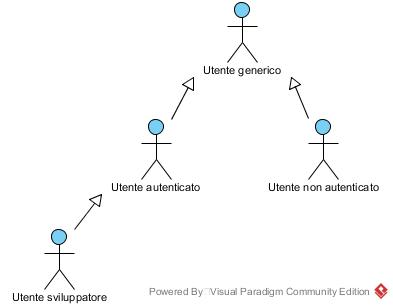
\includegraphics[width=9.7cm]{res/img/gerarchiaAttoriPrimari.jpg}
	\caption{Gerarchia attori primari}
\end{figure}

Sono state identificate quattro diverse tipologie di attori primari relazionati tra loro in maniera gerarchica:

\begin{itemize}
	\item \textbf{Utente generico:} utente che ha eseguito il comando per l'avvio dell'applicativo tramite \textit{Etherlesss-cli};
	\item \textbf{Utente non autenticato:} utente che non ha ancora eseguito l'accesso o la registrazione al network \textit{Ethereum\glo} e che dunque non potrà usufruire delle funzionalità dell'applicazione;
	\item \textbf{Utente autenticato:} utente che ha eseguito l'accesso al network \textit{Ethereum\glo} e che potrà eseguire i comandi messi a disposizione del servizio per gli utenti utilizzatori;
	\item \textbf{Utente sviluppatore:} utente che ha la possibilità di eseguire il deploy di funzioni Javascipt proprie, oltre che eseguire le altre funzioni messe a disposizione dagli altri utenti del servizio.
\end{itemize}



\subsection{Elenco dei casi d'uso}

\begin{figure}[h]
	\centering
	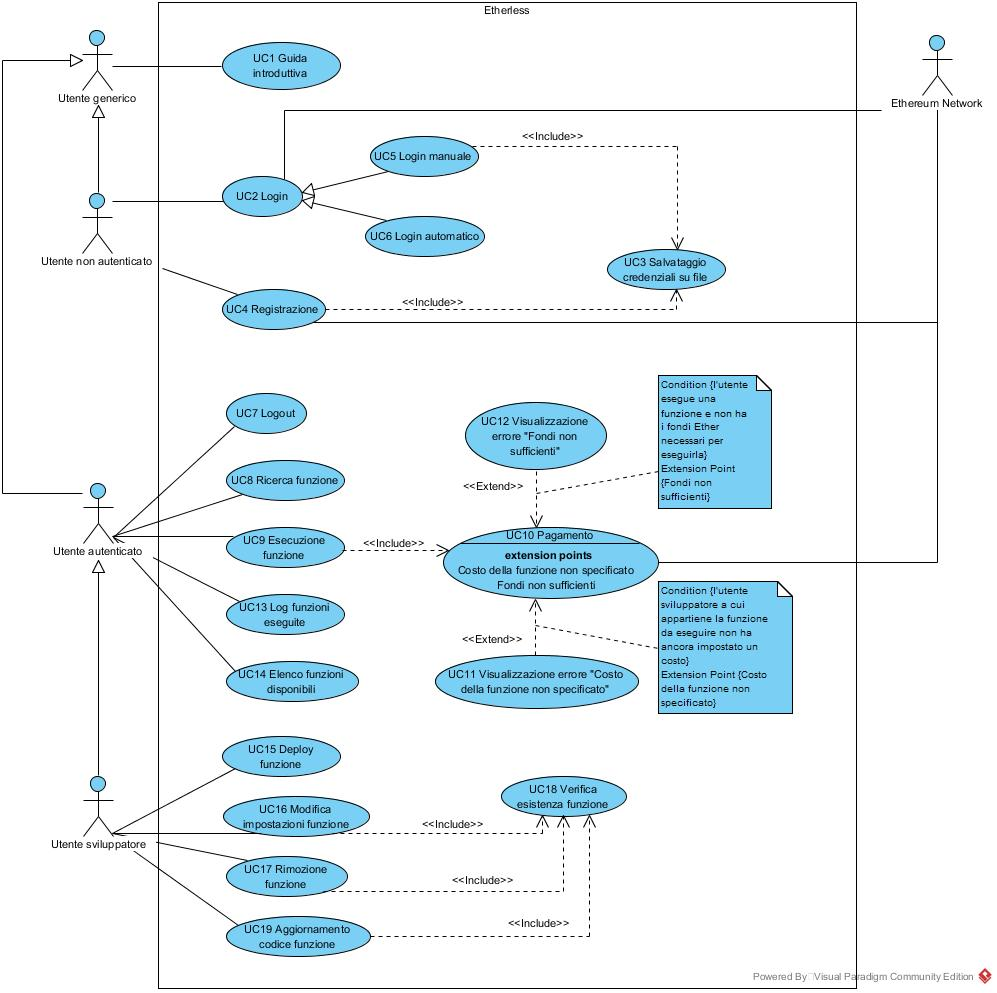
\includegraphics[width=12.3cm]{res/img/useCaseDiagram.jpg}
	\caption{Casi d'uso principali}
\end{figure}
\newpage
\subsubsection{UC1 - Guida introduttiva}
\begin{itemize}
	\item \textbf{Attori primari:} Utente generico;
	\item \textbf{Descrizione:} l'utente generico, appena entrato nell'applicazione, visualizza una guida dei comandi utilizzabili; 
	\item \textbf{Pre-condizioni:} il sistema è raggiungibile e l'applicazione è stata avviata mediante l'apposito comando;
	\item \textbf{Post-condizioni:} Nella \textit{CLI\glo} vengono visualizzati i comandi utilizzabili dall'utente ed una loro descrizione;
	\item \textbf{Scenario principale:} L'utente visualizza la guida introduttiva.
\end{itemize}
\subsubsection{UC2 - Login}
\begin{itemize}
	\item \textbf{Attori primari:} Utente non autenticato;
	\item \textbf{Descrizione:} l'utente ha la possibilità di autenticarsi al network \textit{Ethereum\glo} mediante un address e di una \textit{private key\glos}; 
	\item \textbf{Pre-condizioni:} l'utente ha visualizzato la guida introduttiva e vuole eseguire l'accesso al network \textit{Ethereum};
	\item \textbf{Post-condizioni:} il sistema avrà autenticato o meno l'utente a seconda dei valori di accesso forniti;
	\item \textbf{Scenario principale:} 
	\begin{enumerate}
		\item Vengono inserite le credenziali di accesso (address e \textit{private key\glos}) in maniera manuale o automatica;
		\item L'utente viene autenticato al network \textit{Ethereum\glo} è può usufruire dei comandi messi a disposizione da \textit{Etherless}.
	\end{enumerate}
	\item \textbf{Specializzazioni:}
	\begin{itemize}
		\item \textbf{UC5:} l'utente ha la possibilità di eseguire il login manuale con l'inserimento di address e \textit{private key\glo} da \textit{CLI\glos};
		\item \textbf{UC6:} l'utente verrà automaticamente autenticato dal sistema se presente un file sul proprio dispositivo contenente le credenziali di accesso.  
	\end{itemize}
\end{itemize}
\subsubsection{UC5 - Login manuale}
\begin{figure}[h]
	\centering
	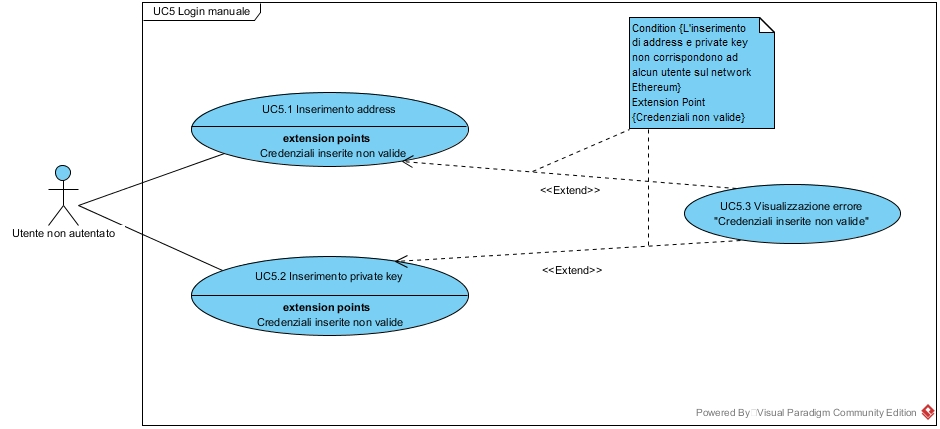
\includegraphics[width=0.8\linewidth]{res/img/UC5.jpg}
	\caption{Diagramma UC5 - Login manuale}
\end{figure}
\begin{itemize}
	\item \textbf{Attori primari:} Utente non autenticato;
	\item \textbf{Descrizione:} l'utente, mediante il comando "login" ha la possibilità di autenticarsi al network \textit{Ethereum\glo} inserendo manualmente da \textit{CLI\glo} il proprio address e \textit{private key\glos} e, contestualmente, salvare in automatico le credenziali di accesso su un file sul proprio dispositivo;
	\item \textbf{Pre-condizioni:} l'utente ha visualizzato la guida introduttiva e desidera autenticarsi manualmente;
	\item \textbf{Post-condizioni:} il sistema avrà autenticato o meno l'utente a seconda dei valori di accesso inseriti dalla \textit{CLI\glos};
	\item \textbf{Scenario principale:}
	\begin{enumerate}
		\item L'utente scriverà un comando da \textit{CLI\glos}, composto nel seguente modo:
		\begin{itemize}
			\item nome del comando "login";
			\item address;
			\item \textit{private key\glos};
			\item password
		\end{itemize}
		\item Verrà visualizzato a schermo un messaggio relativo all'esito dell'autenticazione;
		\item Sarà salvato un file sul dispositivo contenente le credenziali di accesso.
	\end{enumerate}
	\item \textbf{Estensioni:} 
	\begin{itemize}
		\item \textbf{UC5.3}: errore di autenticazione dovuto all'inserimento errato di address/\textit{private key\glos} non corrispondenti ad alcun account \textit{Ethereum\glos}.
	\end{itemize}
\end{itemize}

\subsubsection{UC6 - Login Automatico}
\begin{itemize}
	\item \textbf{Attori primari:} Utente non autenticato;
	\item \textbf{Descrizione:} l'utente, se avrà già effettuato almeno una volta l'accesso alla rete \textit{Ethereum\glo} mediante l'applicazione \textit{Etherless}, potrà accedere automaticamente senza l'inserimento manuale delle credenziali; 
	\item \textbf{Pre-condizioni:} l'utente si è registrato oppure ha eseguito l'accesso almeno una volta mediante \textit{Ethereum};
	\item \textbf{Post-condizioni:} il sistema autenticherà l'utente a seconda dei valori di accesso inseriti nel file;
	\item \textbf{Scenario principale:} se il file è presente nel proprio dispositivo, l'utente avrà la possibilità di utilizzare tutti i comandi disponibili poichè automaticamente autenticato dal sistema. In caso il file risulti assente o corrotto, verrà richiesto il login manuale.
\end{itemize}
\subsubsection{UC4 - Registrazione}
\begin{figure}[h]
	\centering
	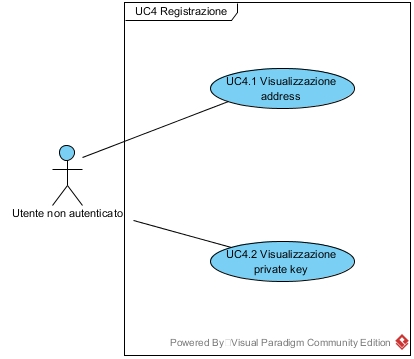
\includegraphics[width=0.7\linewidth]{res/img/UC4.jpg}
	\caption{Diagramma UC4 - Registrazione}
\end{figure}
\begin{itemize}
	\item \textbf{Attori primari:} Utente non autenticato;
	\item \textbf{Attori secondari:} \textit{Ethereum\glo} Network;
	\item \textbf{Descrizione:} l'utente, se non possiede un account \textit{Ethereum\glos}, potrà richiederne uno mediante il comando "signup"; 
	\item \textbf{Pre-condizioni:} l'utente ha visualizzato la guida introduttiva e vuole eseguire la registrazione al network \textit{Ethereum\glos};
	\item \textbf{Post-condizioni:} il sistema registrerà l'utente al network \textit{Ethereum\glo} e lo autenticherà al sistema;
	\item \textbf{Scenario principale:} 
	\begin{enumerate}
		\item L'utente inserisce il comando "signup" per la registrazione;
		\item Il sistema registrerà l'utenza sulla rete \textit{Ethereum\glos};
		\item L'utente risulterà autenticato al sistema;
		\item L'utente potrà vedere le proprie credenziali sulla \textit{CLI\glos};
		\item Sarà salvato un file sul dispositivo contenente le credenziali di accesso.
	\end{enumerate} 
\end{itemize}
\subsubsection{UC7 - Logout}
\begin{itemize}
	\item \textbf{Attori primari:} Utente autenticato;
	\item \textbf{Descrizione:} l'utente autenticato vuole eseguire il logout dal sistema eliminando il file contenente le credenziali di accesso; 
	\item \textbf{Pre-condizioni:} l'utente ha effettuato l'accesso ad \textit{Etherless};
	\item \textbf{Post-condizioni:} verrà eseguito il logout dell'utente autenticato;
	\item \textbf{Scenario principale:} 
	\begin{itemize}
		\item L'utente inserisce il comando per il logout;
		\item Il sistema eseguirà il logout dell'utenza sulla rete \textit{Ethereum\glos} e cancellerà il file di accesso.
	\end{itemize}
\end{itemize}
\subsubsection{UC7 - Ricerca funzione}

\subsubsection{UC9 - Ricerca funzione}
\begin{figure}[h]
	\centering
	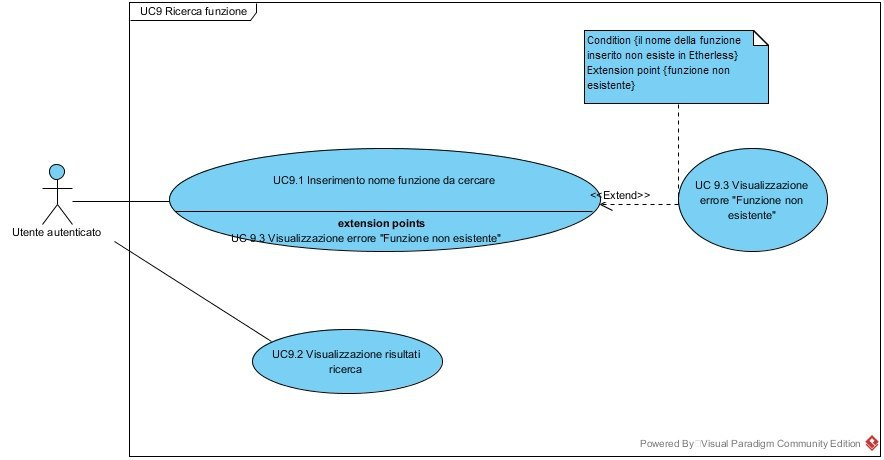
\includegraphics[width=\linewidth]{res/img/UC9.jpg}
	\caption{Diagramma UC9 - Ricerca funzione}
\end{figure}
\begin{itemize}
	\item \textbf{Attori primari:} Utente autenticato;
	\item \textbf{Descrizione:} l'utente autenticato ricerca per nome i dettagli di una specifica funzione caricata da un utente sviluppatore sulla rete \textit{Etherless};
	\item \textbf{Pre-condizioni:} l'utente ha effettuato l'accesso ad \textit{Etherless} e vuole ricercare una funzione specifica mediante l'apposito comando;
	\item \textbf{Post-condizioni:} il sistema visualizzerà a schermo i dettagli della funzione ricercata o un messaggio di errore se la funzione non è stata trovata;
	\item \textbf{Scenario principale:}
	\begin{enumerate}
		\item L'utente scriverà un comando da \textit{CLI\glos} composto nel seguente modo:
		\begin{itemize}
			\item nome del comando "find";
			\item nome della funzione da ricercare.
		\end{itemize}
        \item L'utente visualizzerà la funzione ricercata e i suoi dettagli.
	\end{enumerate}
\end{itemize}

	
\subsection{Tracciamento attori - casi d'uso}	